\documentclass[12pt,a4paper]{article}
\usepackage[utf8]{inputenc}
\usepackage{amsmath}
\usepackage{amsfonts}
\usepackage{amssymb}
\usepackage{lmodern}
\usepackage[toc]{appendix}
\usepackage{graphicx}


%Header packages
\usepackage{fancyhdr}
 %%%%%%%%%%%%%%%%%%%%%%%%%%%%55
 %Might change header back later
\pagestyle{fancy}
\fancyhf{}
\rhead{MAY1607}
\lhead{Microscope HUD}
\rfoot{Page \thepage}




%\author{Noah Bergman}
%\title{Heads-Up Display for a Manufacturing Microscope}




\usepackage{tikz}
\usepackage{epigraph}
\usepackage{lipsum}

\renewcommand\epigraphflush{flushright}
\renewcommand\epigraphsize{\normalsize}
\setlength\epigraphwidth{0.7\textwidth}

\definecolor{titlepagecolor}{cmyk}{1,.60,0,.40}

\DeclareFixedFont{\titlefont}{T1}{ppl}{b}{}{0.5in}

\makeatletter                       
\def\printauthor{%                  
    {\large \@author}}              
\makeatother
\author{%
    \textbf{Prepared By:} \\
    	\begin{flushright}
    		Noah Bergman,\\
    		Greg Kuhn, \\
    		Mike Kelly, \\
    		Garrett Hembry
    	\end{flushright}
%    Department name \\
%    \texttt{email1@example.com}\vspace{20pt} \\
%    Author 2 name \\
 %   Department name \\
%    \texttt{email2@example.com}
    }

% The following code is borrowed from: http://tex.stackexchange.com/a/86310/10898

\newcommand\titlepagedecoration{%
\begin{tikzpicture}[remember picture,overlay,shorten >= -10pt]

\coordinate (aux1) at ([yshift=-15pt]current page.north east);
\coordinate (aux2) at ([yshift=-410pt]current page.north east);
\coordinate (aux3) at ([xshift=-4.5cm]current page.north east);
\coordinate (aux4) at ([yshift=-150pt]current page.north east);

\begin{scope}[titlepagecolor!40,line width=12pt,rounded corners=12pt]
\draw
  (aux1) -- coordinate (a)
  ++(225:5) --
  ++(-45:5.1) coordinate (b);
\draw[shorten <= -10pt]
  (aux3) --
  (a) --
  (aux1);
\draw[opacity=0.6,titlepagecolor,shorten <= -10pt]
  (b) --
  ++(225:2.2) --
  ++(-45:2.2);
\end{scope}
\draw[titlepagecolor,line width=8pt,rounded corners=8pt,shorten <= -10pt]
  (aux4) --
  ++(225:0.8) --
  ++(-45:0.8);
\begin{scope}[titlepagecolor!70,line width=6pt,rounded corners=8pt]
\draw[shorten <= -10pt]
  (aux2) --
  ++(225:3) coordinate[pos=0.45] (c) --
  ++(-45:3.1);
\draw
  (aux2) --
  (c) --
  ++(135:2.5) --
  ++(45:2.5) --
  ++(-45:2.5) coordinate[pos=0.3] (d);   
\draw 
  (d) -- +(45:1);
\end{scope}
\end{tikzpicture}%
}





\begin{document}
%\maketitle
\begin{titlepage}

\noindent
\titlefont Heads-Up Display for a Manufacturing Microscope\par
%\epigraph{Pure mathematics is on the whole distinctly more useful than applied. For what is useful above all is technique, and mathematical technique is taught mainly through pure mathematics.}%
%{\textit{London 1941}\\ \textsc{G. H. Hardy}}
\null
\vspace*{1cm}
\noindent
\begin{minipage}{0.5\textwidth}
    \begin{flushleft}
    \printauthor
    \end{flushleft}
\end{minipage}
%\begin{minipage}{0.1\textwidth}
	%\rule{1pt}{pt}
%\end{minipage}
\vspace{1in}
\\
\begin{minipage}{0.5\textwidth}
    \begin{flushleft}
    \large
    \textbf{Submitted To:}
    	\begin{flushright}
    		\textbf{Bob Dearth}\\
    		Honeywell Intl. Inc. \\
    		~\\
    		\textbf{Dr. Jaeyoun Kim }\\
    		Iowa State University\\
    		~\\
    		\textbf{Dr. George Amariucai}\\
    		Iowa State University
   		\end{flushright}
    \end{flushleft}
\end{minipage}
%
\titlepagedecoration
\end{titlepage}




\pagebreak



\tableofcontents

\listoffigures

\listoftables

\pagebreak
%%%%%%%%%%%%%%%%%%%%%%%%%%%%%%%%%%%%%%%%%%%%%%%%%%%%%%%%%%%%%%%%%%%%%%%%%%%%%%%%%
\section{Introduction}
Honeywell technicians assemble miniature mechanisms under a microscope. They face repetitive movements and eye strain while checking work instructions which are displayed on a nearby computer. A Kansas State design team outlined several solutions to this problem; a small tablet mounted next to the microscope, a virtual environment using technology similar to the Oculus Rift, and a heads up display inside the microscope’s field of view. We are exploring the last of these options. 





%%%%%%%%%%%%%%%%%%%%%%%%%%%%%%%%%%%%%%%%%%%%%%%%%%%%%%%%%%%%%%%%%%%%%%%%%%%%%%
\section{Project Statement}
Optically inserting a virtual screen inside the microscope’s field of view allows the operator to seamlessly refer to work instructions during assembly. This setup could potentially improve workplace ergonomics and reduce manufacturing time while ensuring all components meet Honeywell’s high quality expectations. 

\section{Design Requirements}

\begin{itemize}
	\item Allows users to interact with PDFs that contain embedded pictures, videos, and links to other work instructions.
	\item Does not obstruct the 15” vertical workspace below the objective lens.
	\item Does not restrict airflow in the workspace to maintain ISO Class 7 clean room standards.
	\item Remains in focus during normal microscope operation.
\end{itemize}

\section{Deliverables}
\begin{itemize}
	\item Design working prototype of heads-up display system.
	\item Provide all design documents, schematics, and code.
	\item Operations Manual to demonstrate how to setup and use the system.
	\item Future design manual that outlines improvements and ideas for development down the line.
\end{itemize}


%%%%%%%%%%%%%%%%%%%%%%%%%%%%%%%%%%%%%%%%%%%%%%%%%%%%%%%%%
\section{Functional Overview}
To meet all the requirements, our group designed a DLP projector with custom optics, hardware, and firmware. Our design is centered around the Texas Instruments’ DLP3010 chipset and uses the DLP3010 EVM optical engine and DLP controller board.  The entire system can be broken down into three main parts: main control board, DLP control board, and the optical system. These subsystems work together to display the final image inside the microscope. Figure \ref{block_diagram} shows the block diagram of the final design.

\begin{figure}[h!]
	\centering
	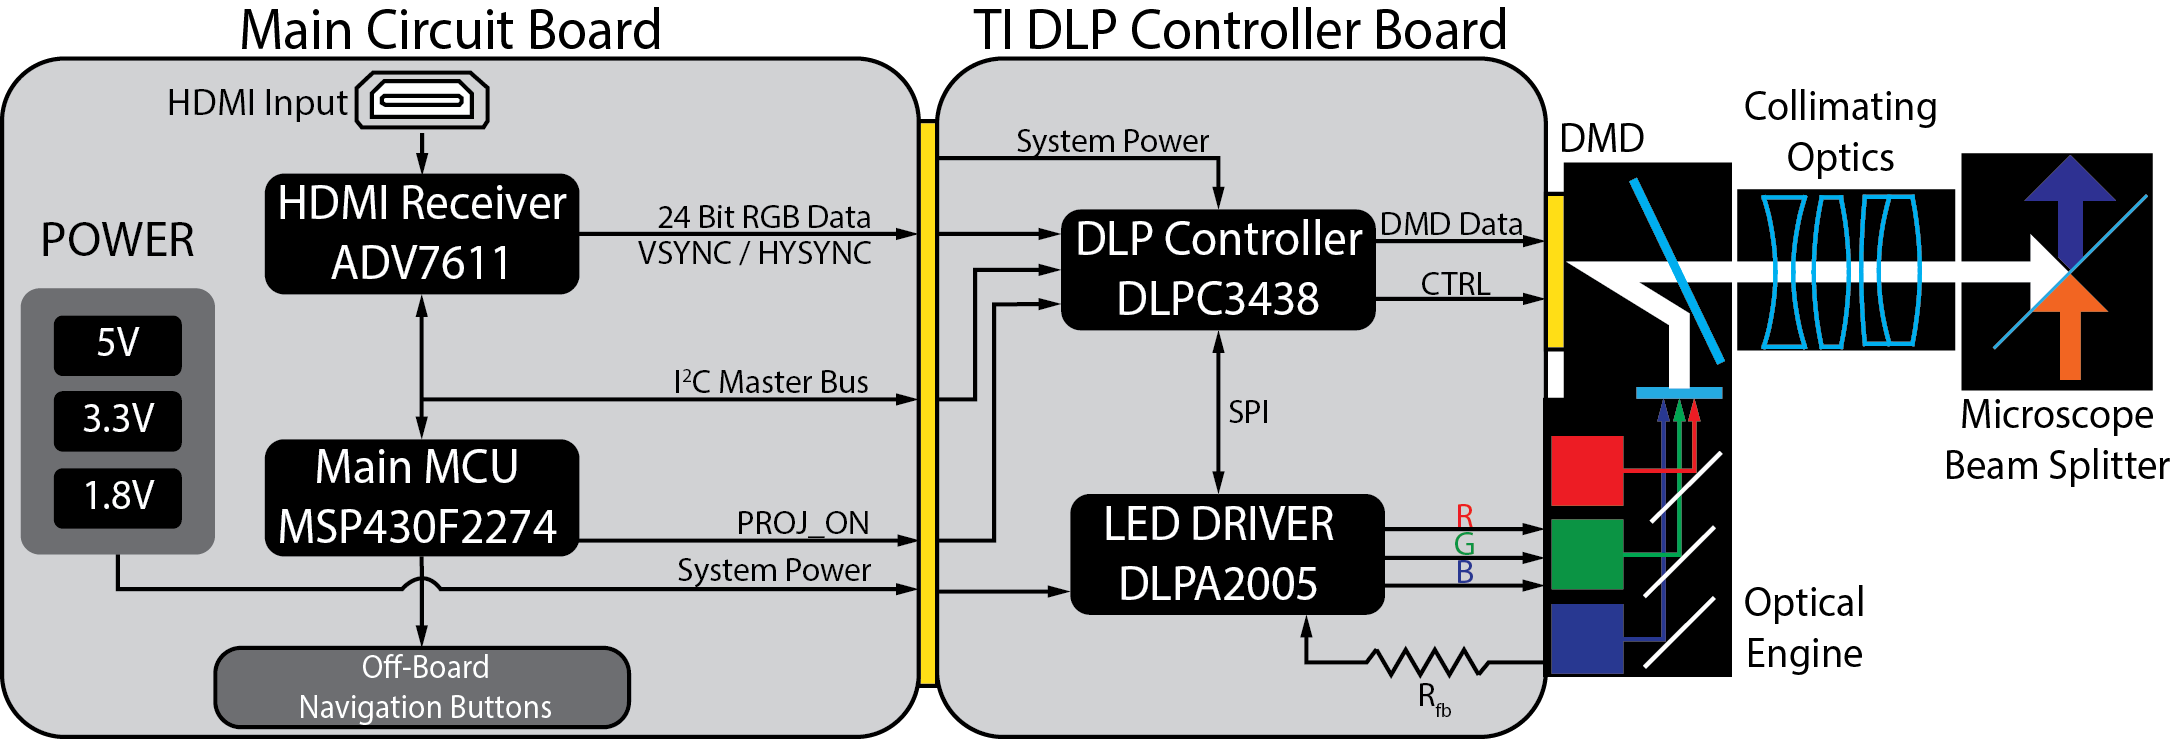
\includegraphics[width = \textwidth]{pics/seniorDesign_blockDiagram.png}
	\caption[Block Diagram]{Block diagram of the main board, DLP controller, and Optical system}
	\label{block_diagram}
\end{figure}


\subsection{Main Control Board}
The main control board was designed to take an HDMI input and convert the data to 24 bit RGB format which is fed directly to the DLP3438 display controller. The on-board microcontroller, MSP430F2274, serves as both a user interface hub and system coordinator. The power-on switch and navigation buttons are connected GPIOs. These inputs are configured in software trigger certain events in the projector. For example, the left and right buttons can be used to change screen size, zoom, and cropping while the power switch simply triggers all the initialization code to run. The MCU communicates with both the ADV7611 and the DLPC3438 over I2C. All the power for the system is routed through the main board. The 5V input is stepped down to 3.3V and 1.8V using buck regulators. 

\subsection{DLP Controller}
The DLP controller board was part of an evaluation kit from Texas Instruments. The board consists of the DLPC3438 display controller and the DLPA2005 PMIC/ LED driver. These two integrated circuits work in tandem to control the DLP3010, digital micro-mirror device.

\subsection{Optical System}
This optical engine uses three LEDs, red, green, and blue, to project a full color image. The light is combined and reflected off the DMD and out through the custom optical system. The optics we designed take the projected light, magnify, correct for aberrations, and finally collimate the image before it is sent into the infinity space of the microscope. The EMZ-8TRU has a camera port attachment that was removed and modified to change the direction of the beam splitter. This allowed the image to be reflected up through the eyepiece where the user can view the virtual screen.




%%%%%%%%%%%%%%%%%%%%%%%%%%%%%%%%%%%%%%%%%%%%%%%%%%%%%%%%%%%%%%%
\section{Detailed Hardware Design}

\subsection{Main Control Board}
\subsubsection{HDMI Receiver - ADV7611}
The ADV7611 receives HDMI signals from the input source, converts the data format, and provides display information to the source over I2C. Before any pixel data can be transferred, the source must know some basic information about the display. The External Device ID is 128 bytes of data that holds manufacturer information, serial number, display dimensions, data speeds, and color information. The final byte holds a check-sum of the data block. Once this information has been transferred over and a confirmation has been sent, both devices are ready to communicate.

The image data is transmitted over four differential pair wires, three for data and one for clock, at 60 frames per second for 1080p displays. This corresponds to a data rate of 3.4Gbps. Routing high speed signals on a circuit board requires special attention. The propagation delay of the signal is directly proportional to the dielectric of fiberglass and length of trace. This becomes incredibly crucial for differential pairs as a mismatch in timing can cause excess power draw on the lines or even corrupt data. 

%%TODO: Fix spacinf!!!!!!!
\begin{equation}
	V_{signal}  = \frac{ 3 \times 10^{8} }{\sqrt{\epsilon_r}}  \mathrm{ , where }\epsilon_r = 4.6 \mathrm{for FR4 PCB material.}  
\end{equation}
%%%%%%%%%%%%%%%%%%%%%%%%%%%%%%%%%%%%%%%%%%%
%Add equation for propagation delay
%
%%%%%%%%%%%%%%%%%%%%%%%%%%%%%%%%%%%%%%%%%%%

%%Insert tolerance for trace matching
%Schematic

The ADV7611 converts the video into 24 bit RGB format. This parallel interface uses 8 bits per color per pixel. Each pixel is clocked in like a typewriter, each pixel placed to right of the previous. At the end of each line, the HSYNC line is pulsed, notifying the receiver to start the next line. The last row of pixels is clocked in and followed by a pulse on the VSYNC line. The receiver sets up for the next frame in the same manner as before, starting in the corner and clocking across.



\subsubsection{Microcontroller - MSP430F2274}
The on-board MSP430F2274 acts as the main coordinator for the system. The DLP controller and ADV7611 are both controlled via I2c. All settings and events are routed through the microcontroller and sent to the respective chip. 
%%%% Add schematic

\subsubsection{Power}
Finally, the main board acts as the power distribution center. The 5V system power is converted to 1.8V and 3.3V using two switching regulators. All three control voltages are necessary for normal operation. When power is first applied, the system waits for the 5V and 3.3V power to stabilize before turning on the 1.8V supply. This power-up sequence is necessary for a clean program start and ensures none of the components are damaged. 
%%% Add schematic

%%%%%%%%%%%%%%%%%%%%%%%%%%%%%%%%%%%%%%%%%%%%5
\subsection{DLP Controller Board}








%Double check on keeping here or in appendix -- The first design is
%not mentioned before this section -- necessarily
\section{Concept Comparison}

Add content to figure out

\section{Testing}
Talk about the cuddly bricks



\section{Recommendations}

Tell engineers to keep moving forward

-Start software for DLPC3438

-Redesign considerations

	 --- Develop other interface for computer
	 
	 --- Develop better interface for projector to use
	  zoom and other functionality
	  
	  
	 

- easier focusing
- 



\section{Conclusion}






%Begin the appendix
\begin{appendices}

\section{Operation Manual}


step 1: go home.

\section{Alternative Designs}



\section{Other Considerations}


\end{appendices}
\end{document}